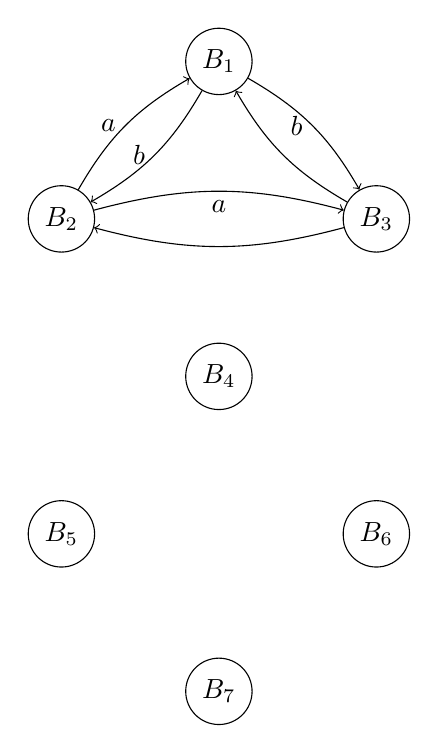
\begin{tikzpicture}
    \node[shape=circle,draw=black] (B1) at (0,0) {$B_1$};
    \node[shape=circle,draw=black] (B2) at (-2,-2) {$B_2$};
    \node[shape=circle,draw=black] (B3) at (2,-2) {$B_3$};
    \node[shape=circle,draw=black] (B4) at (0,-4) {$B_4$};
    \node[shape=circle,draw=black] (B5) at (-2,-6) {$B_5$};
    \node[shape=circle,draw=black] (B6) at (2,-6) {$B_6$};
    \node[shape=circle,draw=black] (B7) at (0,-8) {$B_7$};

    \path [->] (B1) edge[bend left=15] node[left] {$b$} (B2);
    \path [->] (B2) edge[bend left=15] node[left] {$a$} (B1);
    
    \path [->] (B1) edge[bend left=15] node[left] {$b$} (B3);
    \path [->] (B3) edge[bend left=15] node[left] {$\varnothing$} (B1);
    
    \path [->] (B3) edge[bend left=15] node[above] {$\varnothing$} (B2);
    \path [->] (B2) edge[bend left=15] node[below] {$a$} (B3);

\end{tikzpicture}